\chapter{Pendolo su carrello}\label{PendCarrello}
\section{Modello e relative equazioni}\label{equazioni}
\begin{figure}[ht]
	\centering
	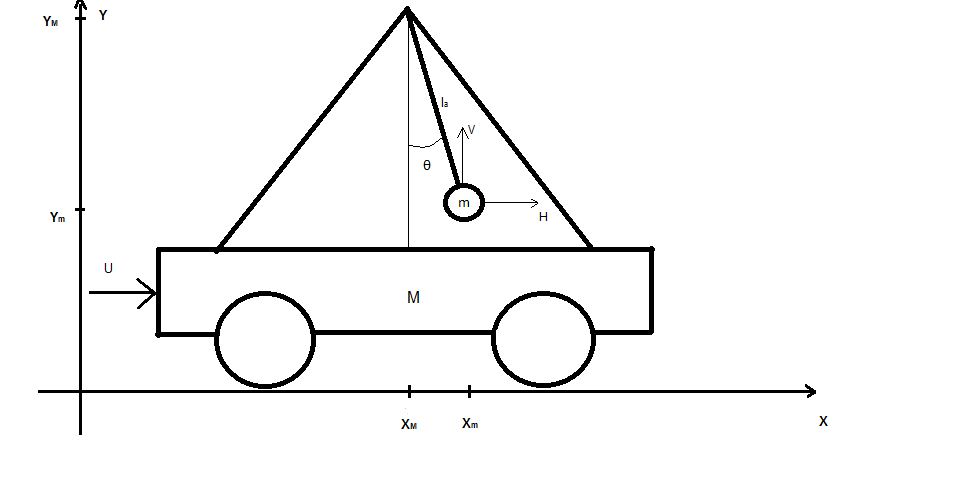
\includegraphics[width=\textwidth]{pendolo.png}\\
	\caption{Modello del pendolo su carrello}
	\label{pendolo}
\end{figure}
\noindent\textbf{Bilanciamento forze sull'asta}\\
Eseguiamo di seguito, sfruttando la Seconda Legge di Newton, il computo delle forze agenti sulla massa $m$ del pendolo lungo entrambi gli assi cartesiani.\\\\
Asse X:
\begin{equation}\notag
m\ddot{x}_m=H
\end{equation}
Asse Y:
\begin{equation}\notag
m\ddot{y}_m=V-mg
\end{equation}
Dove $H$ e $V$ sono le reazioni vincolari (orizzontale e verticale) a cui è sottoposta la massa $m$ per il fatto di essere bloccata all'estremità dell'asta.\\\\
Essendo poi:\\
\begin{equation}\notag
x_m = x_M+l_a\sin(\theta) \quad \Rightarrow \quad \ddot{x}_m=\ddot{x}_M-l_a\sin(\theta)\dot{\theta}^2+l_a\cos(\theta)\ddot{\theta}
\end{equation}
\begin{equation}\notag
y_m=y_M-l_a\cos(\theta) \quad \Rightarrow \quad \ddot{y}_m=l_a\sin(\theta)\ddot{\theta}+l_a\cos(\theta)\dot{\theta}^2
\end{equation}
si ottiene:
\begin{equation}\label{Hv}
H=m\ddot{x}_M-ml_a\sin(\theta)\dot{\theta}^2+ml_a\cos(\theta)\ddot{\theta}
\end{equation}
\begin{equation}\label{Vv}
V=mg+ml_a\cos(\theta)\dot{\theta}^2+ml_a\sin(\theta)\ddot{\theta}
\end{equation}\\
\textbf{Bilanciamento forze sul carrello}\\
Richiamando nuovamente la Legge sopracitata si ha:
\begin{equation}\notag
M\ddot{x}_M=u-H
\end{equation}
da cui sostituendo la \ref{Hv}:
$$
M\ddot{x}_M=u-m\ddot{x}_M+ml_a\sin(\theta)\dot{\theta}^2-ml_a\cos(\theta)\ddot{\theta}
$$
\begin{equation}\label{FCarr}
(M+m)\ddot{x}_M+ml_a\cos(\theta)\ddot{\theta}=u+ml_a\dot{\theta}^2\sin(\theta)
\end{equation}\\
\textbf{Bilanciamento momenti del sistema asta-massa}\\
In questo caso utilizziamo la versione angolare della solita Legge:
\begin{equation}
I_m\ddot{\theta}=l_aV\sin(\theta)+l_aH\cos(\theta)
\end{equation}
sostituendo la \ref{Hv} e la \ref{Vv}:
$$
I_m\ddot{\theta}=l_a\sin(\theta)[mg+ml_a\cos(\theta)\dot{\theta}^2+ml_a\sin(\theta)\ddot{\theta}]+$$$$+l_a\cos(\theta)[m\ddot{x}_M-ml_a\sin(\theta)\dot{\theta}^2+ml_a\cos(\theta)\ddot{\theta}]=
$$
$$
=mgl_a\sin(\theta)+ml_a^2\sin(\theta)\cos(\theta)\dot{\theta}^2+ml_a^2\sin^2(\theta)\ddot{\theta}+ml_a\ddot{x}_M\cos(\theta)+$$$$-ml_a^2\cos(\theta)\sin(\theta)\dot{\theta}^2
+ml_a^2\cos^2(\theta)\ddot{\theta}=$$
$$=mgl_a\sin(\theta)+ml_a^2\ddot{\theta}+ml_a\ddot{x}_M\cos(\theta) =
$$
\begin{equation} \label{momInThetaP}
=ml_a(g\sin(\theta)+l_a\ddot{\theta}+\ddot{x}_M\cos(\theta))
\end{equation}
Essendo il momento d'inerzia dell'asta $$
I_a=\displaystyle\frac{1}{12}m_al_a^2+m_a(\displaystyle\frac{l}{2})^2=\displaystyle\frac{1}{3}m_al_a^2=0.000045kg\cdot m^2$$molto inferiore (1 ordine di grandezza) rispetto a quello della massa $m$ attaccata al pendolo: $$
I_m=ml_a^2=0.00041kg\cdot m^2$$ possiamo per semplicità trascurarlo, per cui poniamo $I_m=0$.

Il sistema che deriva dalla \ref{FCarr} e dalla \ref{momInThetaP} è dunque il seguente:
\\\\
$\begin{cases}
$$(M+m)\ddot{x}_M+ml_a\cos(\theta)\ddot{\theta}=u+ml_a\dot{\theta}^2\sin(\theta)$$ \\
$$g\sin(\theta)+l_a\ddot{\theta}+\ddot{x}_M\cos(\theta)=0$$\\
\end{cases}
$
\\\\
Dalla prima equazione del sistema: 
$$
(M+m)(\frac{-g\sin(\theta)-l_a\ddot{\theta}}{\cos(\theta)})+ml_a\cos(\theta)\ddot{\theta}=u+ml_a\dot{\theta}^2\sin(\theta)
$$
$$
\ddot{\theta}(ml_a\cos(\theta)-\frac{l_a(M+m)}{\cos(\theta)}=u+ml_a\dot{\theta}^2\sin(\theta)+\frac{g\sin(\theta)(M+m)}{\cos(\theta)}
$$
$$
\ddot{\theta}=\frac{[u+ml_a\dot{\theta}^2\sin(\theta)+\displaystyle\frac{g\sin(\theta)(M+m)}{\cos(\theta)}]\cos(\theta)}{ml_a\cos^2(\theta)-l_a(M+m)} \Rightarrow$$\\
\begin{equation}\label{theta2punti}
\ddot{\theta}=\frac{u\cos(\theta)+ml_a\dot{\theta}^2\sin(\theta)\cos(\theta)+g\sin(\theta)(M+m)}{-l_a(m\sin^2(\theta)+M)}
\end{equation}\\
Dalla seconda equazione del sistema:
$$
\ddot{x}_M=\frac{-g\sin(\theta)-l_a\ddot{\theta}}{\cos(\theta)}
$$
e sostituendo ora la \ref{theta2punti}:  
$$
\ddot{x}_M=\frac{-g\sin(\theta)-\displaystyle\frac{ul_a\cos(\theta)+ml^2_a\dot{\theta}^2\sin(\theta)\cos(\theta)+gl_a\sin(\theta)(M+m)}{-l_a(m\sin^2(\theta)+M)}}{\cos(\theta)}=
$$
$$
=\frac{g\sin(\theta)[-l_a(m\sin^2(\theta)+M)]+ul_a\cos(\theta)+ml^2_a\dot{\theta}^2\sin(\theta)\cos(\theta)+gl_a\sin(\theta)(M+m)}{l_a\cos(\theta)(m\sin^2(\theta)+M)}=
$$
$$
=\frac{-gm\sin^3(\theta)-gM\sin(\theta)+u\cos(\theta)+ml_a\dot{\theta}^2\sin(\theta)\cos(\theta)+gM\sin(\theta)+gm\sin(\theta)}{\cos(\theta)(m\sin^2(\theta)+M)}
$$
$$
=\frac{u+ml_a\dot{\theta}^2\sin(\theta)+gm\cos(\theta)\sin(\theta)}{m\sin^2(\theta)+M}
$$
\newpage
Assegniamo le variabili di stato e definiamo le uscite desiderate:\\\\
$\begin{cases}
$$x_1 \stackrel{\Delta}{=} x_M$$ \\
$$x_2\stackrel{\Delta}{=}\dot{x}_M$$\\
$$x_3\stackrel{\Delta}{=}\theta$$\\
$$x_4\stackrel{\Delta}{=}\dot{\theta}$$\\
$$y_1\stackrel{\Delta}{=}x_M$$ \\
$$y_2\stackrel{\Delta}{=}\theta$$\\
\end{cases}
$\\\\\\
Sostituendo queste ultime nelle equazioni appena ricavate si ottengono le equazioni:
\\\\\\
$\underline{\dot{x}}=\displaystyle\frac{d}{d t}
\begin{bmatrix}
x_M\\\\
\dot{x}_M\\\\
\theta\\\\
\dot{\theta}\\\\
\end{bmatrix}
=
\begin{bmatrix}
x_2\\\\
\displaystyle\frac{u+ml_ax_4^2\sin(x_3)+gm\cos(x_3)\sin(x_3)}{m\sin^2(x_3)+M}\\\\
x_4\\\\
-\displaystyle\frac{u\cos(x_3)+ml_ax_4^2\sin(x_3)\cos(x_3)+g(M+m)\sin(x_3)}{l_a(m\sin^2(x_3)+M)}\\\\
\end{bmatrix}
$
\\\\\\
\section{Linearizzazione del modello}\label{LinMod}
\textbf{Punti di equilibrio del sistema} \\
Per la ricerca dei punti di equilibrio poniamo $\underline{f}(\underline{x},u)=\underline{0}$\quad(dove $\underline{\dot{x}}=\underline{f}(\underline{x},u$)) da cui:\\\\
$\begin{cases}
$$x_2=0$$ \\
$$\displaystyle\frac{u+ml_ax_4^2\sin(x_3)+gm\cos(x_3)\sin(x_3)}{m\sin^2(x_3)+M}=0$$\\
$$x_4=0$$\\
$$\displaystyle\frac{u\cos(x_3)+ml_ax_4^2\sin(x_3)\cos(x_3)+g(M+m)\sin(x_3)}{l_a(m\sin^2(x_3)+M)}=0$$
\end{cases}
$\\\\\\
Dal precedente sistema si può notare che punti di equilibrio del pendolo su carrello sono due, uno instabile per \\
$\begin{cases}
$$x_1=\forall$$ \\
$$x_2=0$$\\
$$x_3=\pm\pi$$\\
$$x_4=0$$\\
$$u=0$$
\end{cases}$\\\\
ovvero quando il pendolo è rivolto verso l'alto (pendolo inverso), l'altro, stabile, per\\
$\begin{cases}
$$x_1=\forall$$ \\
$$x_2=0$$\\
$$x_3=0$$\\
$$x_4=0$$\\
$$u=0$$
\end{cases}$\\\\
quando il pendolo è rivolto verso il basso (pendolo "normale"), caso da noi trattato nel seguito.\\
In ultimo, siccome il punto di equilibrio non dipende dalla posizione del carrello, possiamo per semplicità scegliere $x_1=0$.\\\\
\textbf{Linearizzazione del sistema attorno al punto di equilibrio}\\
Vogliamo ora linearizzare le precedenti equazioni di stato attorno al punto di equilibrio $\underline{\tilde{x}}=\underline{0}$, $\tilde{u}=0$ trovato: \\\\
$\displaystyle\frac{\partial{f_1}}{\partial{\underline{x}}}(\underline x,u)=
\begin{bmatrix}
0&1&0&0
\end{bmatrix}$\qquad
$\displaystyle\frac{\partial{f_1}}{\partial{u}}(\underline{x},u)=0$\\\\\\
$\displaystyle\frac{\partial{f_2}}{\partial{x_1}}(\underline{x},u)=0$\qquad
$\displaystyle\frac{\partial{f_2}}{\partial{x_2}}(\underline{x},u)=0$\\
$\displaystyle\frac{\partial{f_2}}{\partial{x_3}}(\underline{x},u)=\displaystyle\frac{[ml_ax_4^2\cos(x_3)+mg(\cos^2(x_3)-\sin^2(x_3))](M+m\sin^2(x_3))}{(M+m\sin^2(x_3))^2}$\\
$-\displaystyle\frac{[u+ml_ax_4^2\sin(x_3)+mg\sin(x_3)\cos(x_3)](2\sin(x_3)\cos(x_3))}{(M+m\sin^2(x_3))^2}\bigg|_{\underline{\tilde{x}},\tilde{u}}=\displaystyle\frac{mg}{M}$\\ $\displaystyle\frac{\partial{f_2}}{\partial{x_4}}(\underline{x},u)=\displaystyle\frac{2ml_a\sin(x_3)x_4}{M+m\sin^2(x_3)}\bigg|_{\underline{\tilde{x}},\tilde{u}}=0$\\
$\displaystyle\frac{\partial{f_2}}{\partial{u}}(\underline{x},u)=\displaystyle\frac{1}{M+m\sin^2(x_3)}\bigg|_{\underline{\tilde{x}},\tilde{u}}=\displaystyle\frac{1}{M}$\\\\\\
$\displaystyle\frac{\partial{f_3}}{\partial{\underline{x}}}(\underline x,u)=
\begin{bmatrix}
0&0&0&1
\end{bmatrix}$\qquad$\displaystyle\frac{\partial{f_3}}{\partial{u}}(\underline{x},u)=0$\\\\\\
$\displaystyle\frac{\partial{f_4}}{\partial{x_1}}(\underline{x},u)=0$\qquad
$\displaystyle\frac{\partial{f_4}}{\partial{x_2}}(\underline{x},u)=0$\\
$\displaystyle\frac{\partial{f_4}}{\partial{x_3}}(\underline{x},u)=$\\$\displaystyle\frac{[u\sin(x_3)-ml_ax_4^2(\cos^2(x_3)-\sin^2(x_3))-g\cos(x_3)(M+m)][l_a(m\sin^2(x_3)+M)]}{l_a^2(m\sin^2(x_3)+M)^2}+$ $-\displaystyle\frac{[-u\cos(x_3)-ml_ax^2_4\sin(x_3)\cos(x_3)-g\sin(x_3)(m+M)][2ml_a\sin(x_3)\cos(x_3)]}{l_a^2(m\sin^2(x_3)+M)^2}\bigg|_{\underline{\tilde{x}},\tilde{u}}=$
$=-\displaystyle\frac{(M+m)g}{Ml}$\qquad$\displaystyle\frac{\partial{f_4}}{\partial{x_4}}(\underline{x},u)=\displaystyle\frac{-2ml_ax_4\sin(x_3)\cos(x_3)}{l_a(m\sin^2(x_3)+M)}\bigg|_{\underline{\tilde{x}},\tilde{u}}=0$\\$\displaystyle\frac{\partial{f_4}}{\partial{u}}(\underline{x},u)=\displaystyle\frac{-\cos(x_3)}{l_a(m\sin^2(x_3)+M)}\bigg|_{\underline{\tilde{x}},\tilde{u}}=-\displaystyle\frac{1}{ml_a}$\\\\\\
Le equazioni di stato linearizzate sono dunque:\\\\
$\underline{\delta\dot{x}}=
\begin{bmatrix}
0&1&0&0\\
0&0&\displaystyle\frac{mg}{M}&0\\
0&0&0&1\\
0&0&-\displaystyle\frac{(M+m)g}{Ml_a}&0
\end{bmatrix}
\underline{\delta x}+
\begin{bmatrix}
0\\
\displaystyle\frac{1}{M}\\
0\\
-\displaystyle\frac{1}{Ml_a}\\
\end{bmatrix}
\underline{\delta u}
$\\\\
$\underline{\delta y}=
\begin{bmatrix}
1&0&0&0\\
0&0&1&0
\end{bmatrix}
\underline{\delta x}
$\\\\\\
Calcolando ora la funzione di trasferimento $T_{y_2,u}$ tra l'ingresso $u$ (forza esercitata sul carrello,
avanti/indietro) e l'uscita $y_2$(angolo $\theta$ del pendolo rispetto alla verticale) si ottiene:\\\\
$T_{y_2,u}(s)=C(sI-A)^{-1}B=
\begin{bmatrix}
0&0&1&0
\end{bmatrix}
\begin{bmatrix}
*&*&*&*\\
*&*&*&*\\
*&0&*&\displaystyle\frac{1}{s^2+\frac{(M+m)g}{Ml_a}}\\
*&*&*&*
\end{bmatrix}
\begin{bmatrix}
0\\
\displaystyle\frac{1}{M}\\
0\\
-\displaystyle\frac{1}{Ml_a}\\
\end{bmatrix} = \\
=-\displaystyle\frac{1}{Ml_as^2+(M+m)g}
$\\\\
in cui il segno meno è coerente col fatto che il semiperiodo iniziale dell'oscillazione del pendolo sia in direzione opposta rispetto al movimento del carrello.

Inserendo ora i parametri del modello fisico del pendolo su  carrello realizzato con l'ausilio del LEGO MINDSTORMS EV3 si può procedere all'identificazione della funzione di trasferimento.
\begin{table}[ht]
	\begin{tabular}{|l|l|l|l|}
		\hline
		\textbf{Sigla} & \textbf{Valore} & \textbf{U.d.m.} & \textbf{Parametro}\\
		\hline
		$M$ & 0.7535 & $kg$ & massa carrello\\
		\hline
		$m$ & 0.016 & $kg$ & massa all'estremità del pendolo\\
		\hline
		$g$ & 9.81 & $m/s^2$ & accelerazione di gravità\\
		\hline
		$l_a$ & 0.166 & $m$ & lunghezza asta del pendolo\\
		\hline
		$r$ & 0.034 & $m$ & raggio ruote motrici\\
		\hline
	
	\end{tabular}	
\caption{Parametri del sistema Carrello-Pendolo}
\label{carrPend}
\end{table}
\\Data la tabella \ref{carrPend} si ha:
$$T_{y_2,u}(s)=-\displaystyle\frac{1}{0.125s^2+7.541}$$
\newpage
\section{Stabilizzazione del pendolo}\label{stabPend}
Il pendolo di per sé è un sistema già stabile; lo scopo della realizzazione su carrello consiste nello smorzarne l'oscillazione riducendo la costante di tempo e quindi il transitorio del sistema grazie all'impiego di due ruote motrici.\\
In figura \ref{pendoloFisico} si può vedere la realizzazione del pendolo su carrello utilizzando un motore EV3 Large Servo Motor come trazione e un encoder GlideWheel-M per misurare l'angolo del pendolo 
\begin{figure}[ht]
	\centering
	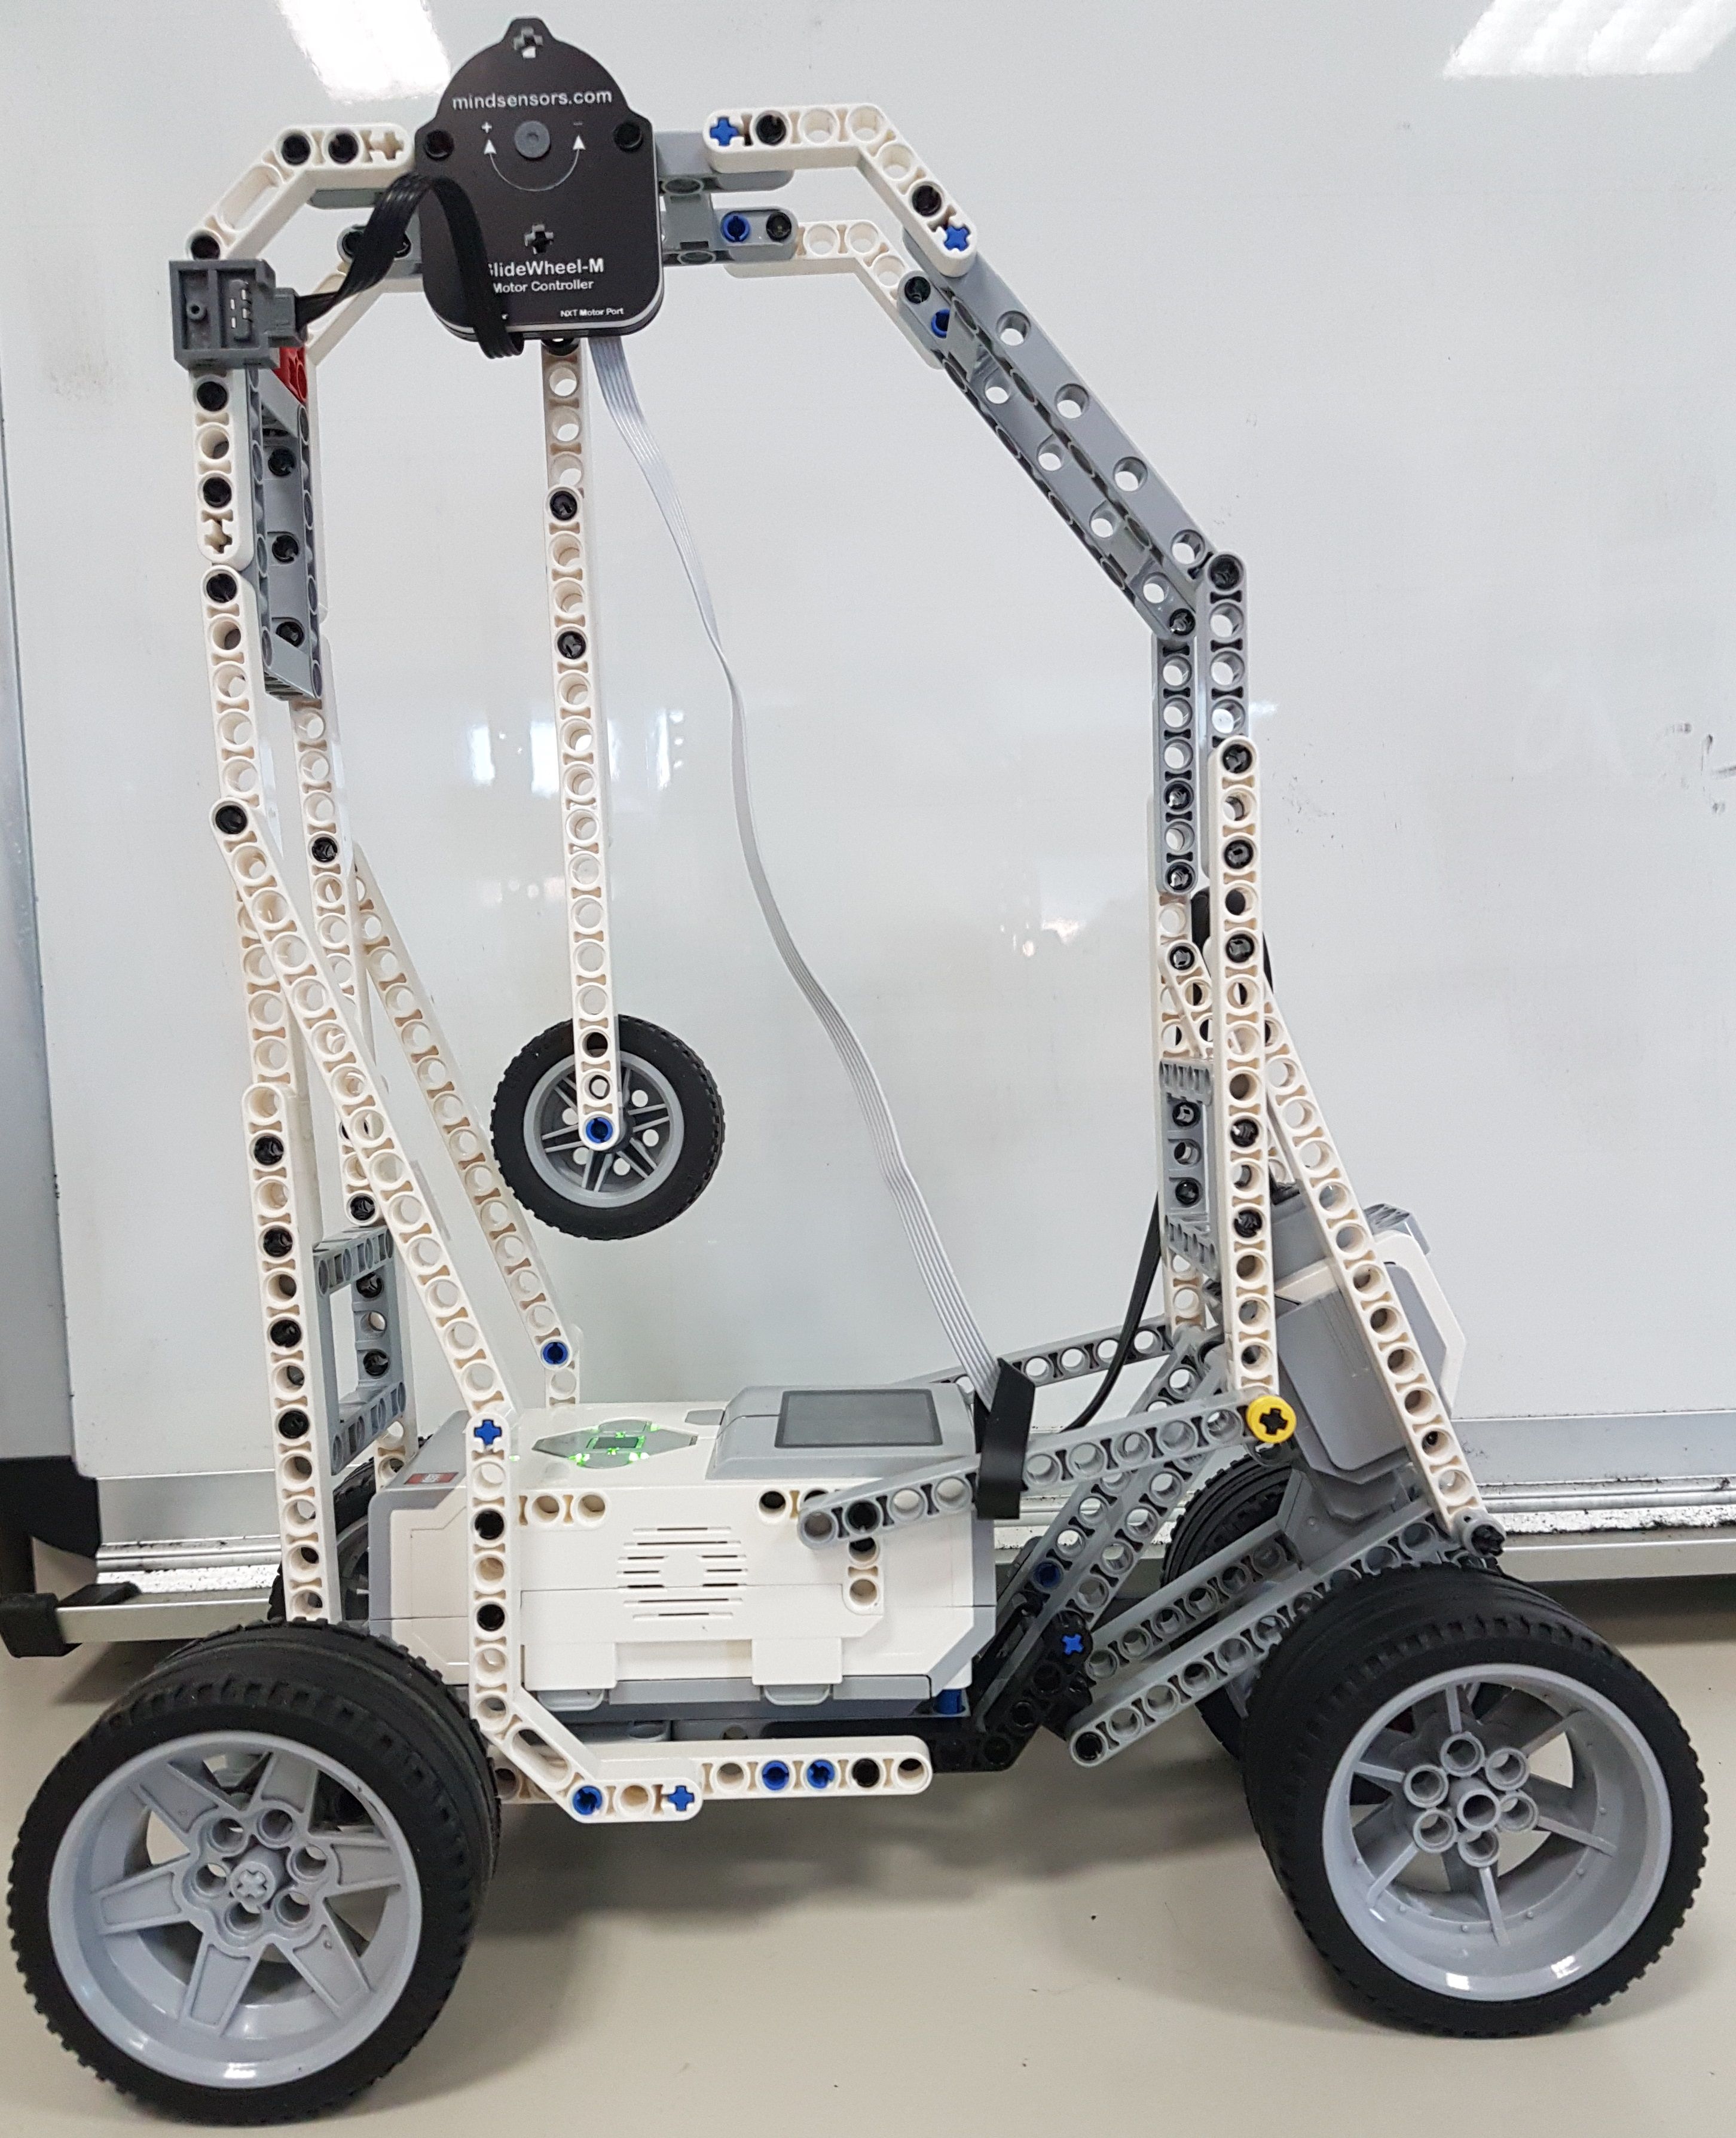
\includegraphics[scale=0.08]{pendoloFisico.jpg}\\
	\caption{Realizzazione fisica del pendolo su carrello}
	\label{pendoloFisico}
\end{figure} 
rispetto alla verticale.\\

Da specifiche tale encoder è in grado di raggiungere un tempo di campionamento minimo di $0.001s$ (così come il motore) col quale non si riesce sempre a campionare in modo corretto. Per ovviare, almeno parzialmente, al problema abbiamo deciso di abbassare la frequenza di campionamento, in modo però da non perdere nessuna variazione dell'angolo del pendolo.\\
Per fare questo abbiamo calcolato la massima velocità raggiunta durante la sua oscillazione libera tra $[\ang{-31},\ang{+31}]$ (intervallo entro il quale il pendolo è vincolato per costruzione).
\begin{figure}[ht]
	\centering
	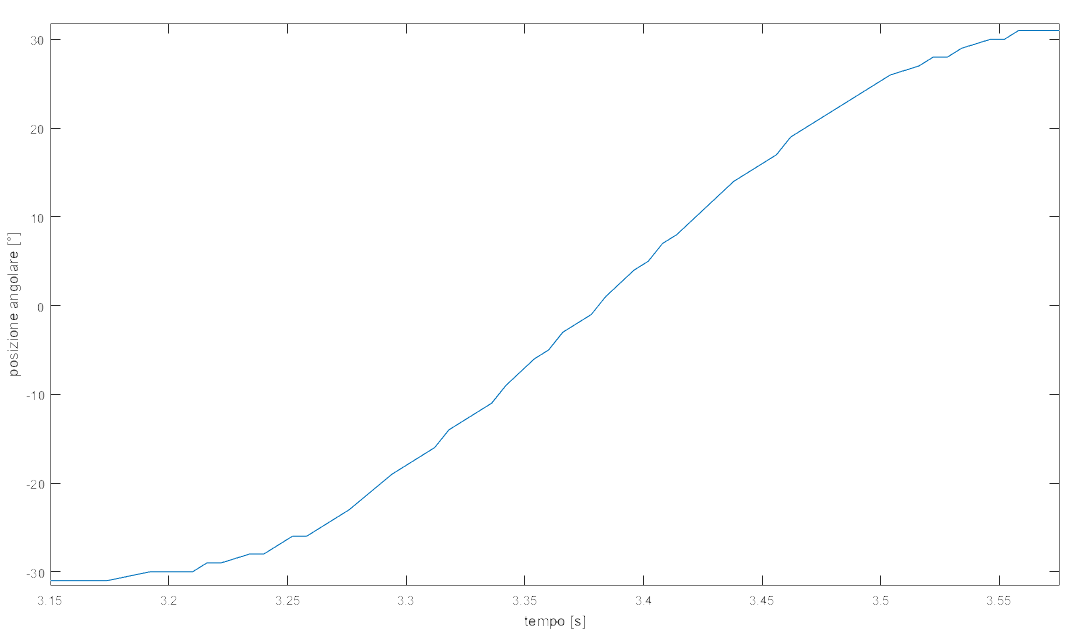
\includegraphics[width=\textwidth]{SlewRate.PNG}\\
	\caption{Massima velocità di oscillazione libera}
	\label{slewRate}
\end{figure}
\\Da tale esperimento è risultato che durante la prima oscillazione (in figura \ref{slewRate}), il pendolo, raggiunge per $\theta=\ang{0}$ la velocità $\omega=250\deg/s$ (calcolata con un semplice rapporto incrementale) per cui il tempo di campionamento necessario a non perdere nessuna variazione dell'angolo sarebbe stato $t_c=\displaystyle\frac{1}{250}=0.004s$.\\

Sfruttando il modello del motore LEGO da noi identificato al capitolo \ref{modMotor} si può quindi ricavare la funzione di trasferimento del sistema complessivo (avente come ingresso la potenza richiesta al motore e come uscita la posizione angolare del pendolo).\begin{figure}[ht]
	\centering
	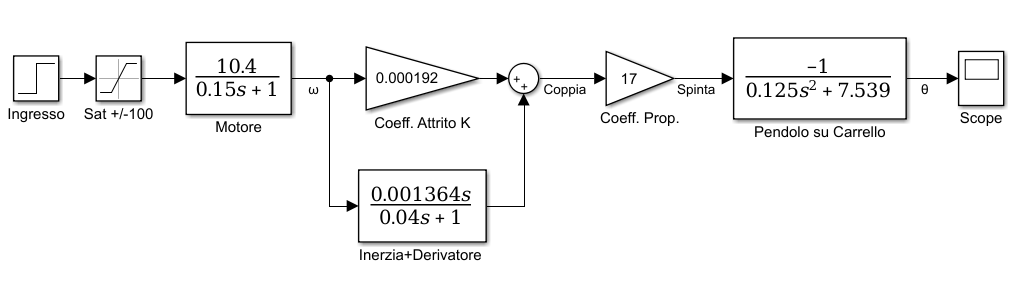
\includegraphics[width=\textwidth]{SisComplessivoPendoloNormale.PNG}
	\caption{Schema a blocchi del sistema complessivo}
	\label{SisComplessivoPendoloNormale}
\end{figure}

Siccome in uscita al modello del motore abbiamo la coppia erogata dallo stesso, per poterlo mettere in serie al modello del pendolo su carrello (il quale come ingresso riceve una spinta sotto forma di forza) occorre adattare il collegamento I/O. Poiché si assume un moto di puro rotolamento delle ruote del carrello, si tratta di trovare il giusto coefficiente $C$ di proporzionalità tra coppia e spinta.
\begin{figure}[ht]
	\centering
	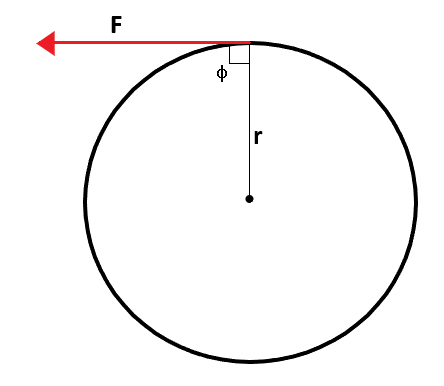
\includegraphics[scale=0.55]{braccioForza.PNG}
	\caption{Momento della forza applicato alla ruota}
	\label{braccioForza}
\end{figure}
\\La relazione tra queste ultime è data dalla formula fisica del momento della forza:
$$\tau=r\times F=(r\sin(\phi))F=r_{\bot}F$$
ove $r_{\bot}$ rappresenta il braccio della forza F.
Poiché nel nostro caso $r$ risulta essere il raggio della ruota ed F la forza tangente alla ruota abbiamo ricavato, sostituendo il suo valore dalla tabella \ref{carrPend}: $$F=\displaystyle\frac{\tau}{r}\Rightarrow$$$$\Rightarrow C=\displaystyle\frac{1}{r}=29.41$$

Per realizzare ora una retroazione algebrica sull'uscita che ci permetta di controllare il pendolo in ciclo chiuso, possiamo riassumere in un'unica funzione di trasferimento il sistema complessivo.\\
Per farlo ci siamo serviti del `Linear Analisys Tool' di Simulink che, tra le altre cose, può essere utilizzato per ricostruire la funzione di trasferimento tra due punti specificati di un sistema (nel nostro caso tra l'ingresso del motore e l'uscita $\theta$).
$$T_{y_2,u}=-\displaystyle\frac{559.5s+78.3}{s^4+31.67s^3+227s^2+1910s+10050}$$

Tra i principali modi per studiarne la stabilità in ciclo chiuso uno dei più noti è il luogo delle radici, il quale permette di verificare lo spostamento dei poli al variare del guadagno.\\
Quello che si prova a fare è spostare tutti i poli in ciclo chiuso nel semipiano destro, mantenendoli possibilmente vicini all'asse Reale.
Questo perché se nei poli predomina la parte Immaginaria essi introdurranno maggiore oscillazione nell'assestamento della risposta del sistema. 

Come si evince dal luogo delle radici del sistema, è possibile utilizzare un semplice regolatore Proporzionale purché il suo guadagno rientri in un intervallo molto limitato, ovvero $P\in(-6,0)$.
\begin{figure}[ht]
	\centering
	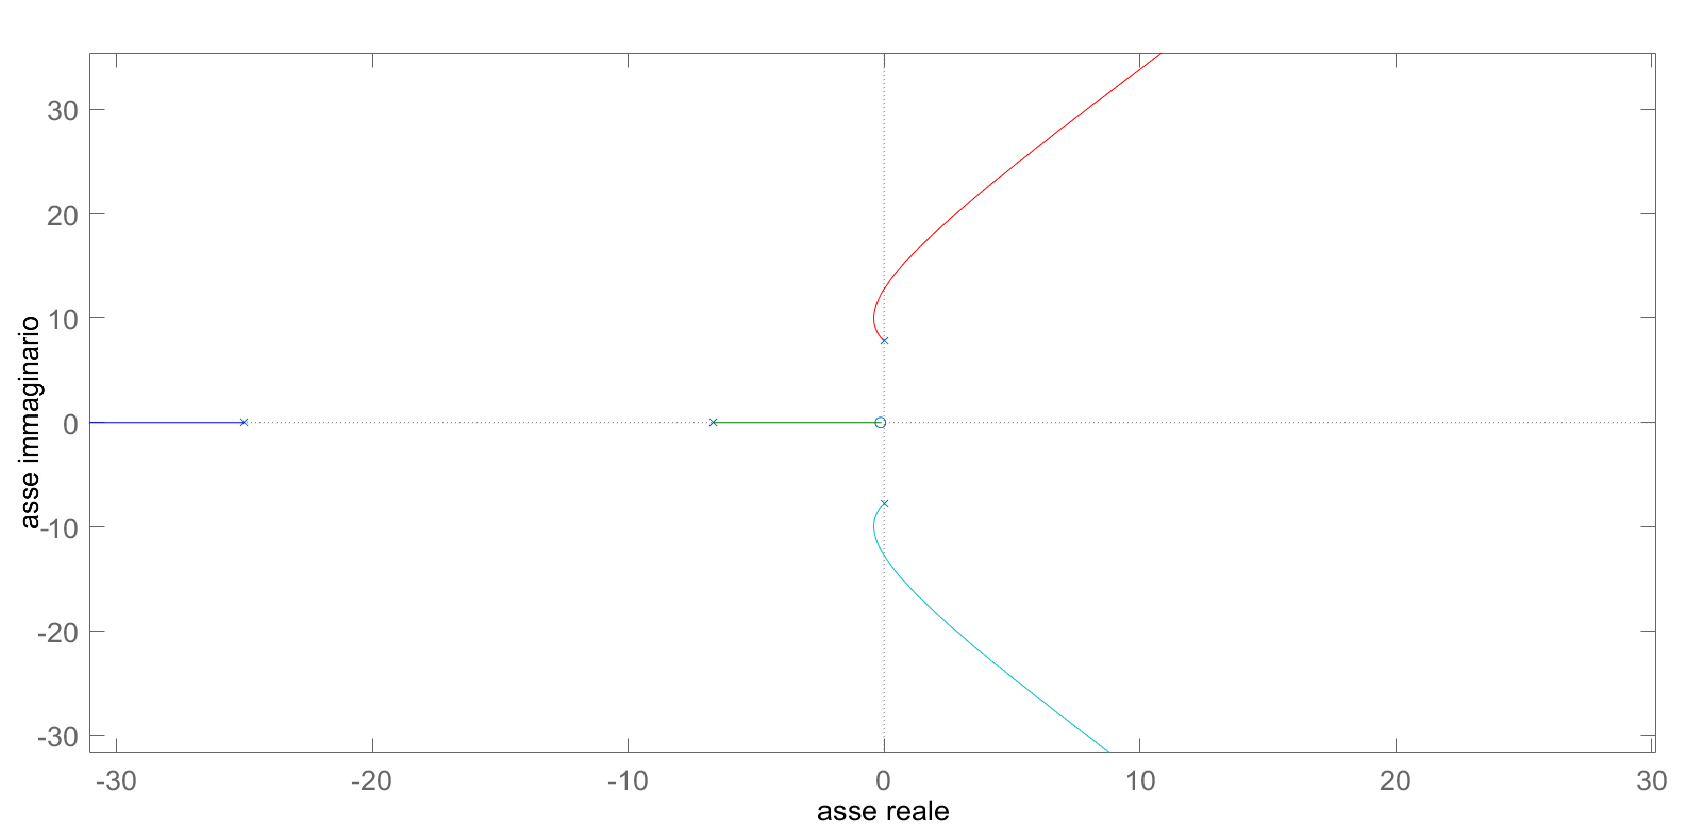
\includegraphics[width=\textwidth]{RLocusPendoloNormale.PNG}
	\caption{Luogo delle Radici di $-T_{y_2,u}$}
	\label{RLocusPendoloNormale}
\end{figure}
\\Attraverso l'utilizzo dello strumento MATLAB chiamato `rlocus', il quale consente di ottenere data una funzione il luogo delle radici, siamo arrivati a definirne il guadagno $P=-2$ (vedi figura \ref{gainOttimaleft}) come ottimale, dato il massimo rapporto possibile tra parte Reale e parte Immaginaria, in ciclo chiuso, dei due poli complessi coniugati .
\begin{figure}[ht]
	\centering
	\includegraphics[width=\textwidth]{gainOttimaleft.PNG}
	\caption{Particolare del Luogo delle Radici di $-T_{y_2,u}$}
	\label{gainOttimaleft}
\end{figure}
\\Tale valore è stato in seguito validato dall'analisi della risposta del sistema  durante la simulazione attraverso diversi esperimenti, i cui risultati saranno mostrati nel seguito.
\begin{figure}[ht]
	\centering
	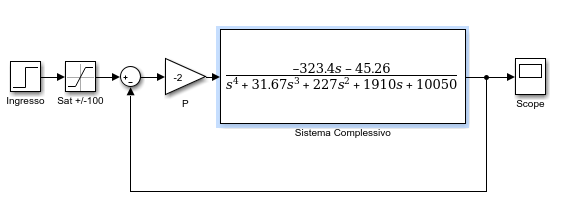
\includegraphics[width=\textwidth]{SisComplessivoPNRetroazionato.PNG}
	\caption{Sistema complessivo controllato proporzionalmente}
	\label{SisComplessivoPNRetroazionato}
\end{figure}
\\Nella realizzazione dello schema a blocchi in Simulink, caricato nel Brick EV3 MINDSTORMS per confermare la veridicità dei risultati ottenuti, abbiamo posto un ingresso costante a 0 poiché si assume il pendolo inizialmente a riposo nel punto di equilibrio $\theta=\ang{0}$.
\begin{figure}[ht]
	\centering
	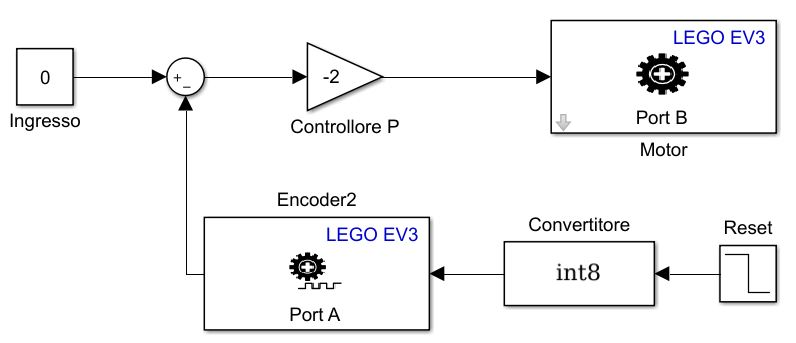
\includegraphics[width=\textwidth]{pendoloReale.jpg}
	\caption{Sistema reale controllato proporzionalmente}
	\label{pendoloReale}
\end{figure}
\\L'encoder, invece, è settato a $0$ tramite un segnale di reset dopo un tempo pari a $0.001s$ dall'inizializzazione poiché, all'avvio del programma caricato nel Brick, viene considerato come angolo $\theta=\ang{0}$ di riferimento il primo valore misurato.
Per effettuare tale operazione è necessario inserire nello schema un convertitore dal momento che il GlideWheel-M richiede in ingresso unicamente un segnale di tipo `int8' (interi a 8 bit), mentre il blocco di reset ne genera uno `double' a 64 bit in accordo con lo standard IEEE 754.\\
Sotto tali presupposti il motore, avendo ingresso nullo, non erogherà potenza fino quando il pendolo non verrà spostato dal suo stato iniziale.\\
Al variare della posizione angolare, il motore reagirà muovendo il carrello nella stessa direzione per riportare il pendolo nel suo punto di equilibrio.

Come accennato poco fa, ad ulteriore conferma della veridicità del luogo delle radici, abbiamo provato a controllare il sistema fisico al variare di $P$ durante una simulazione interattiva, nella quale è possibile modificare in tempo reale, da PC, il valore del guadagno del regolatore, e, come mostrato nella figura \ref{variazioneGainP}, il sistema risulta effettivamente instabile per valori che si discostano dall'intervallo di stabilità trovato.\\
L'esperimento è così costituito: avviato il programma nel Brick siamo noi ad innescare la prima oscillazione nel pendolo in modo da osservarne il comportamento. Nel caso in cui esso non riesca a ritornare nel punto di equilibrio autonomamente allora siamo noi a fermarlo.
\begin{figure}[ht]
	\centering
	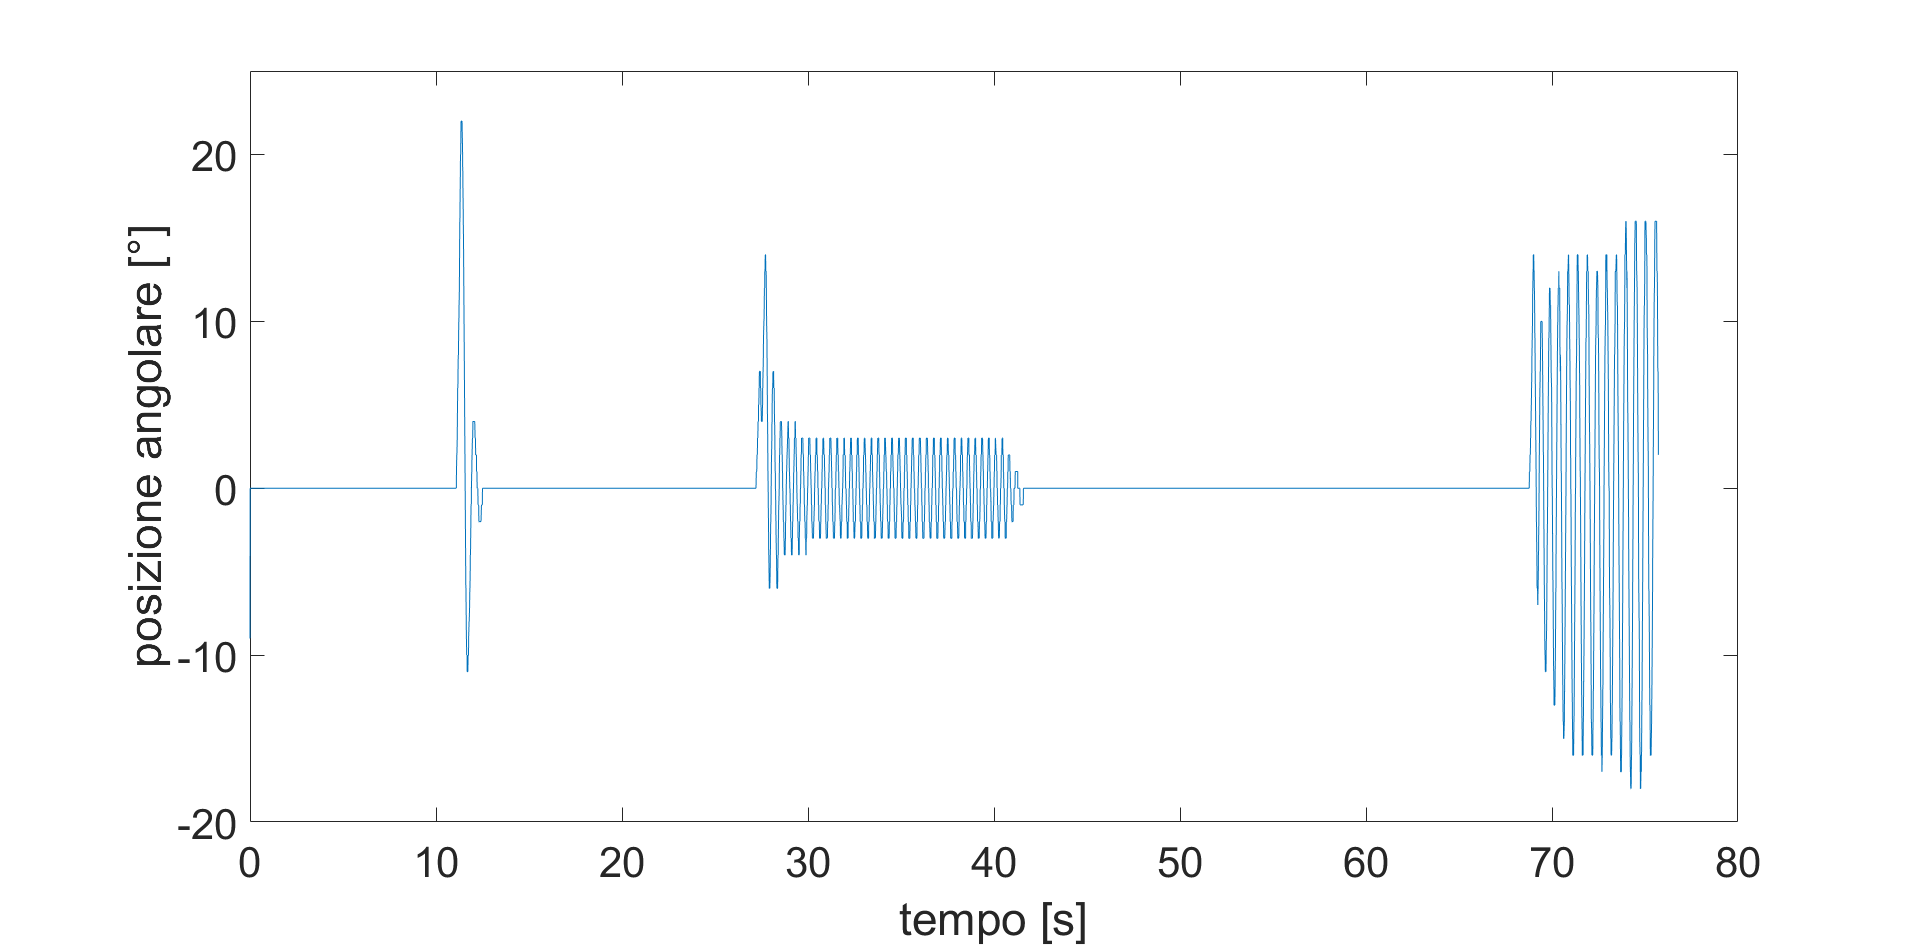
\includegraphics[width=\linewidth]{variazioneGainP.png}
	\caption{Uscita $\theta$ del sistema per valori di $P=-2,-6,-8$}
	\label{variazioneGainP}
\end{figure}
\begin{itemize}
	\item Nell'intervallo tra $10s$ e $15s$ ($P=-2$) è chiaro come il pendolo ritorni nel punto di equilibrio quasi immediatamente.
	\item Tra $25s$ e $40s$ ($P=-6$), in seguito ad uno smorzamento iniziale non riesce a ritornare nel punto di equilibrio, ma continua ad oscillare fino al nostro intervento.
	\item Tra $70s$ e $80s$ ($P=-8$), non avviene nemmeno uno smorzamento iniziale ma anzi, l'oscillazione provocata viene amplificata dal sistema fino a giungere in una situazione nella quale le ipotesi del modello vengono violate: le ruote del carrello iniziano a slittare, inficiando dunque le equazioni trovate al paragrafo \ref{stabPend} che si basavano sul moto di puro rotolamento.
\end{itemize}

Assodato quindi come $P=-2$ porti ad una situazione più che accettabile, si è cercato di quantificare il miglioramento raggiunto tra sistema in ciclo aperto e sistema in ciclo chiuso con retroazione unitaria.\\
Come si può vedere nel grafico in figura \ref{oscillOL}, posizionando il pendolo ad un'angolazione di $\theta=\ang{31}$ (massima raggiungibile per costruzione) e lasciandolo quindi libero di oscillare, in ciclo aperto
\begin{figure}[ht]
	\centering
	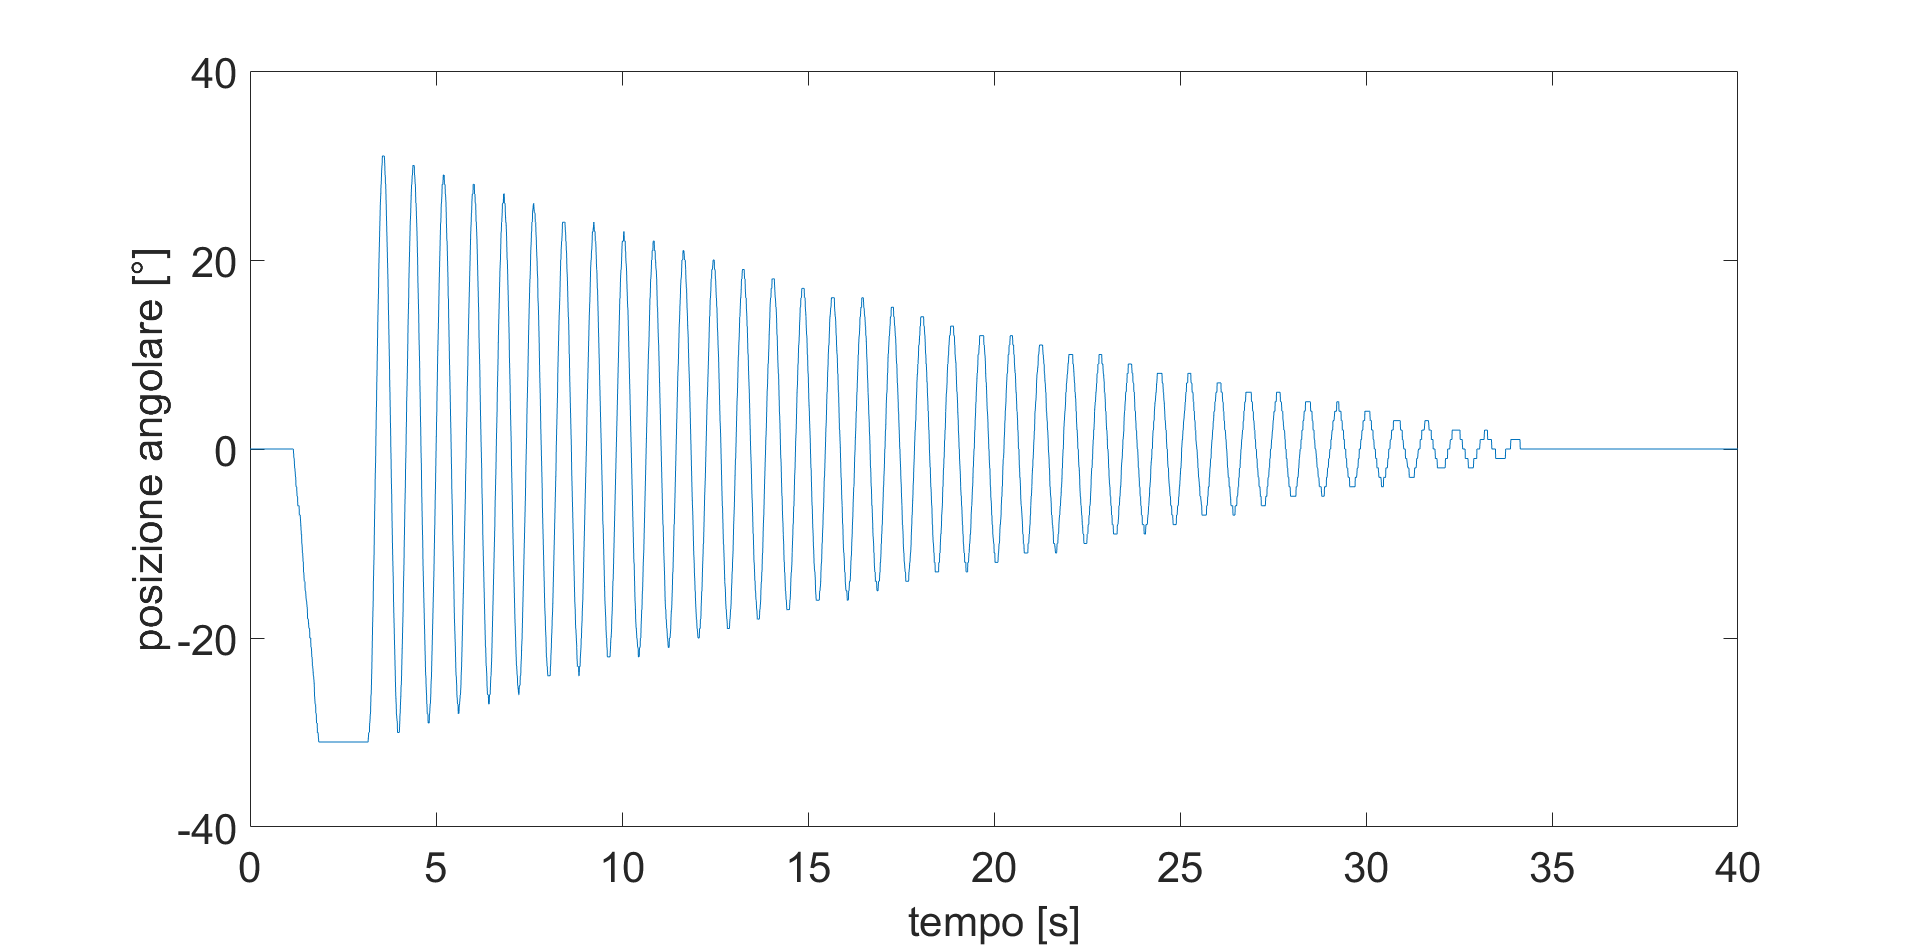
\includegraphics[width=\linewidth]{oscillOL.PNG}
	\caption{Sistema in ciclo aperto}
	\label{oscillOL}
\end{figure}
 (ovvero senza controllo sul motore) si raggiunge il punto di stabilità $\theta=\ang{0}$ in poco più di $30$ secondi, mentre risulta un tempo di appena $1.4$ secondi per quanto riguarda il sistema in ciclo chiuso.
\begin{figure}[ht]
	\centering
	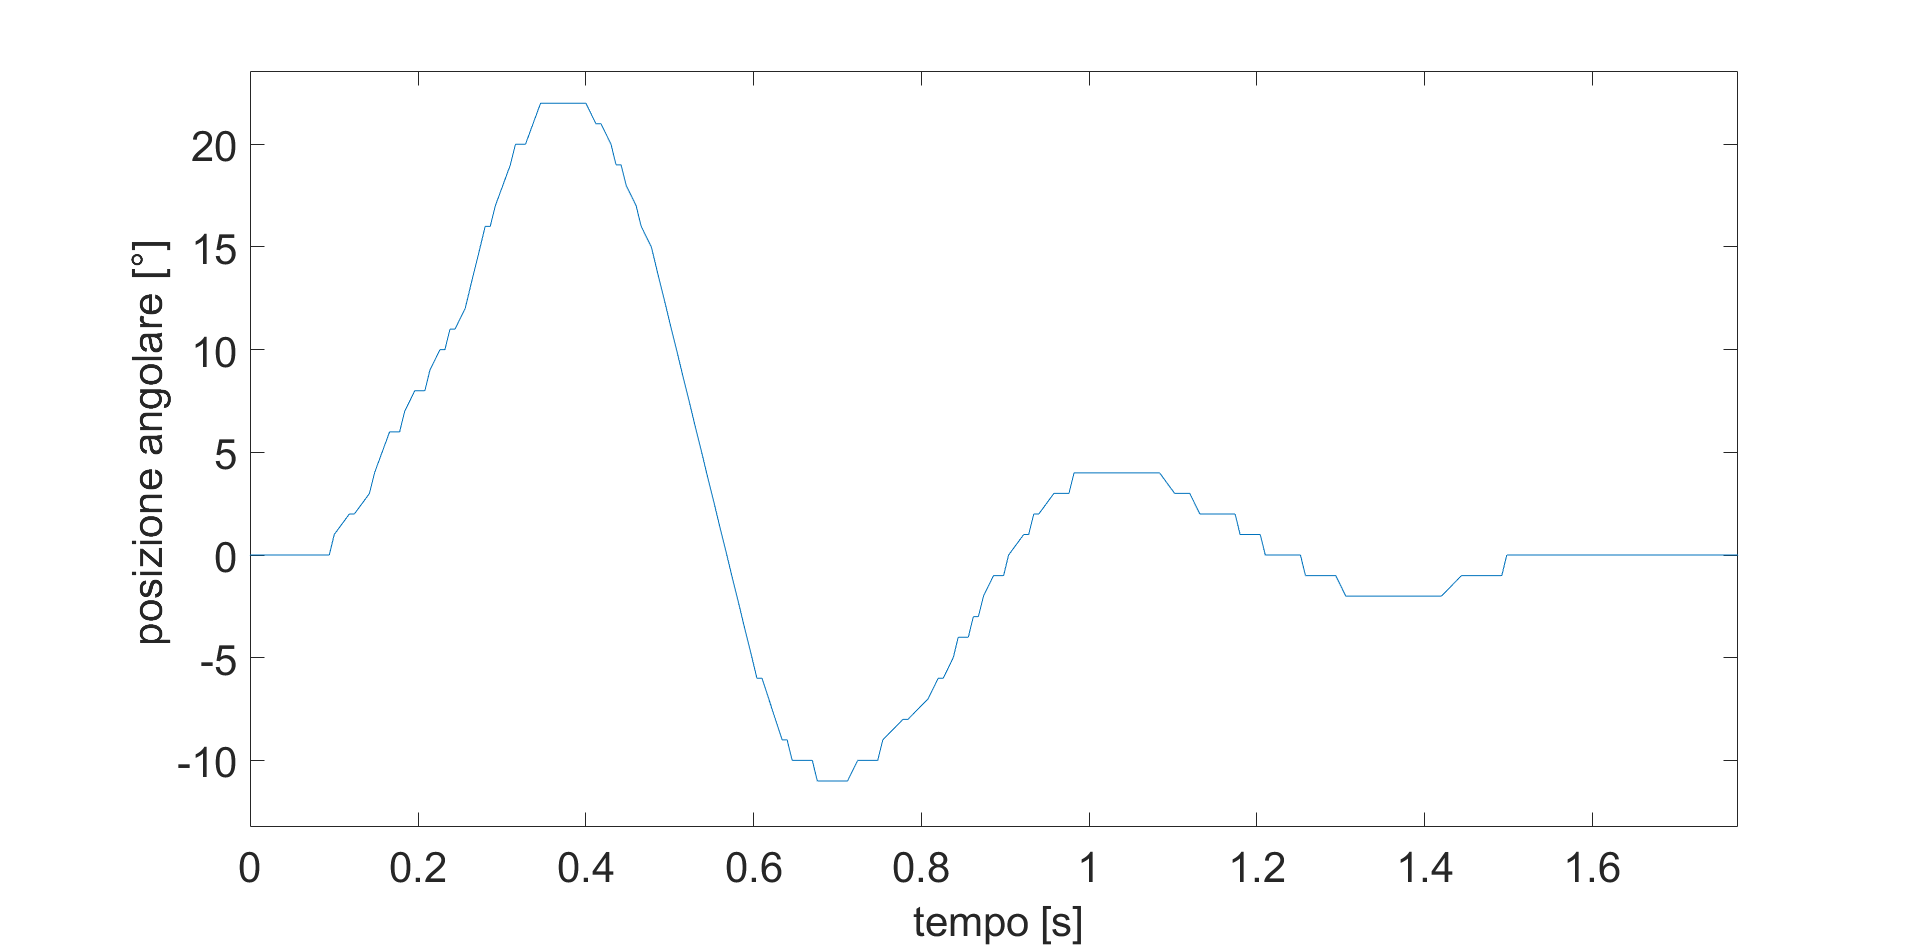
\includegraphics[width=\linewidth]{oscillCL.PNG}
	\caption{Sistema in ciclo chiuso con Regolatore P}
	\label{oscillCL}
\end{figure} 


